\documentclass{article}
\usepackage[utf8x]{inputenc}
\usepackage{ucs}
\usepackage{amsmath} 
\usepackage{amsfonts}
\usepackage{upgreek}
\usepackage[english,russian]{babel}
\usepackage{graphicx}
\usepackage{float}
\usepackage{textcomp}
\usepackage{hyperref}
\usepackage{geometry}
  \geometry{left=2cm}
  \geometry{right=1.5cm}
  \geometry{top=1cm}
  \geometry{bottom=2cm}
\usepackage{tikz}
\usepackage{ccaption}
\usepackage{multicol}

\usepackage{listings}
%\setlength{\columnsep}{1.5cm}
%\setlength{\columnseprule}{0.2pt}


\begin{document}
\pagenumbering{gobble}

\lstset{
  language=C,                % choose the language of the code
  basicstyle=\linespread{1.1}\ttfamily,
  columns=fixed,
  fontadjust=true,
  basewidth=0.5em,
  keywordstyle=\color{blue}\bfseries,
  commentstyle=\color{gray},
  stringstyle=\ttfamily\color{orange!50!black},
  showstringspaces=false,
  %numbers=false,                   % where to put the line-numbers
  numbersep=5pt,
  numberstyle=\tiny\color{black},
  numberfirstline=true,
  stepnumber=1,                   % the step between two line-numbers.        
  numbersep=10pt,                  % how far the line-numbers are from the code
  backgroundcolor=\color{white},  % choose the background color. You must add \usepackage{color}
  showstringspaces=false,         % underline spaces within strings
  captionpos=b,                   % sets the caption-position to bottom
  breaklines=true,                % sets automatic line breaking
  breakatwhitespace=true,         % sets if automatic breaks should only happen at whitespace
  xleftmargin=.2in,
  extendedchars=\true,
  keepspaces = true,
  frame=tlbr,
  framesep=8pt,
  framerule=0pt,
  xleftmargin=.3\textwidth, 
  xrightmargin=.1\textwidth,
  }
\lstset{literate=%
   *{0}{{{\color{red!20!violet}0}}}1
    {1}{{{\color{red!20!violet}1}}}1
    {2}{{{\color{red!20!violet}2}}}1
    {3}{{{\color{red!20!violet}3}}}1
    {4}{{{\color{red!20!violet}4}}}1
    {5}{{{\color{red!20!violet}5}}}1
    {6}{{{\color{red!20!violet}6}}}1
    {7}{{{\color{red!20!violet}7}}}1
    {8}{{{\color{red!20!violet}8}}}1
    {9}{{{\color{red!20!violet}9}}}1
}

\definecolor{solcolor}{RGB}{226,240,245}

\title{Семинар \#2: Часть 1: Функции. \vspace{-5ex}}\date{}\maketitle
\section*{Функции}
Функция - это сущность, которая ассоциирует с собой набор инструкций и входящие в неё параметры.
Можно использовать функции, написанные другими программистами. Например, вы уже использовали функции
\texttt{printf} и \texttt{scanf} из стандартной библиотеки \texttt{stdio.h}. 

Можно писать и свои функции. В примере ниже была написана функция \texttt{square}, которая принимает одно целое чиисло и возвращает квадрат этого числа. Функция \texttt{square} используется в функции \texttt{main}, чтобы вычислить квадрат числа 5. Чтобы вызвать функцию \texttt{square} нужно написать её имя и сразу после имени в скобках передать одно целое число. Как только программа "увидет" выражение \texttt{square(5)} она зайдёт в функцию \texttt{square}, при этом будет считать что параметр \texttt{x} равен 5. После того как функция выполнится и вернёт число 25, программа подставит за место выражения \texttt{square(5)} число 25.
\begin{lstlisting}
#include <stdio.h>

int square(int x)
{
    return x * x;
}

int main()
{
    printf("%i\n", square(5));
}
\end{lstlisting}



Помимо функций с возвращаемым значением можно написать и функцию, которая ничего не возвращает. Например, \texttt{print\_n\_times} -- печатает число \texttt{n} раз и ничего не возвращает. У функций, которые ничего не возвращают на месте возвращаемого типа стоит ключевое слово \texttt{void}.
\begin{lstlisting}
#include <stdio.h>

void print_n_times(int a, int n) 
{
    for (int i = 0; i < n; ++i)
        printf("%i ", a);
}

int main() 
{
    print_n_times(7, 3);
}
\end{lstlisting}


\subsection*{Задачи:}
Решите задачи в папке \texttt{code/0function}.

\newpage
\section*{Копирование при передаче в функцию}
Одна из самых важных вещей, которые нужно знать о функциях: При передаче в функцию объекты копируются.
Соответственно, функция работает с копией передаваемого объекта.\\

Рассмотрим, например, пример ниже. В функции \texttt{main} мы создаём переменную \texttt{a}, равную 10 и передаём её в функцию \texttt{inc}. Но при передаче в функцию \texttt{inc} переменная \texttt{a} копируется и функция \texttt{inc} работает с копией переменной \texttt{a}. Соответвенно, если мы увеличим на 1 переменную \texttt{a} в функции \texttt{inc}, то переменная \texttt{a} в функции \texttt{main} не поменяется. В результате на экран будет напечатано число 10.


\begin{lstlisting}
#include <stdio.h>

void inc(int a)
{
    a += 1;
}

int main()
{
    int a = 10;
    inc(a);
    printf("%i\n", a);
}
\end{lstlisting}

Единственные объекты, которые не копируются в функции при передаче это массивы. Подробнее о передаче массивов в функции будет чуть позже.

\subsection*{Задачи:}
Решите задачи в папке \texttt{code/1scope}.

\newpage
\section*{Рекурсия}
Рекурсивная функция -- это функция, которая вызывает саму себя.  В примере ниже функция \texttt{counter} -- рекурсивная. Если этой функции передать, скажем, число 4, то она напечатает это число и вызовет функцию \texttt{counter}, передав ей число 3. Новый вызов функции \texttt{counter} с аргументом 3 напечатает 3 и вызовет функцию \texttt{counter}, передав ей число 2. Так будет продолжаться пока число не дойдёт до 0 и сработает проверка \texttt{n <= 0}.
\begin{lstlisting}
#include <stdio.h>

void counter(int n) 
{
    if (n <= 0)
        return;

    printf("%i ", n);
    counter(n - 1);
}

int main() 
{
    counter(4);
}
\end{lstlisting}

Для лучшего понятия, что происходит в этой функциях \texttt{counter} рассмотрим на схемы вызовов рекурсивной функции. Для изначальной функции \texttt{counter} она выглядит следующим образом (предположим, что вызываем \texttt{counter(4)}):


\begin{center}
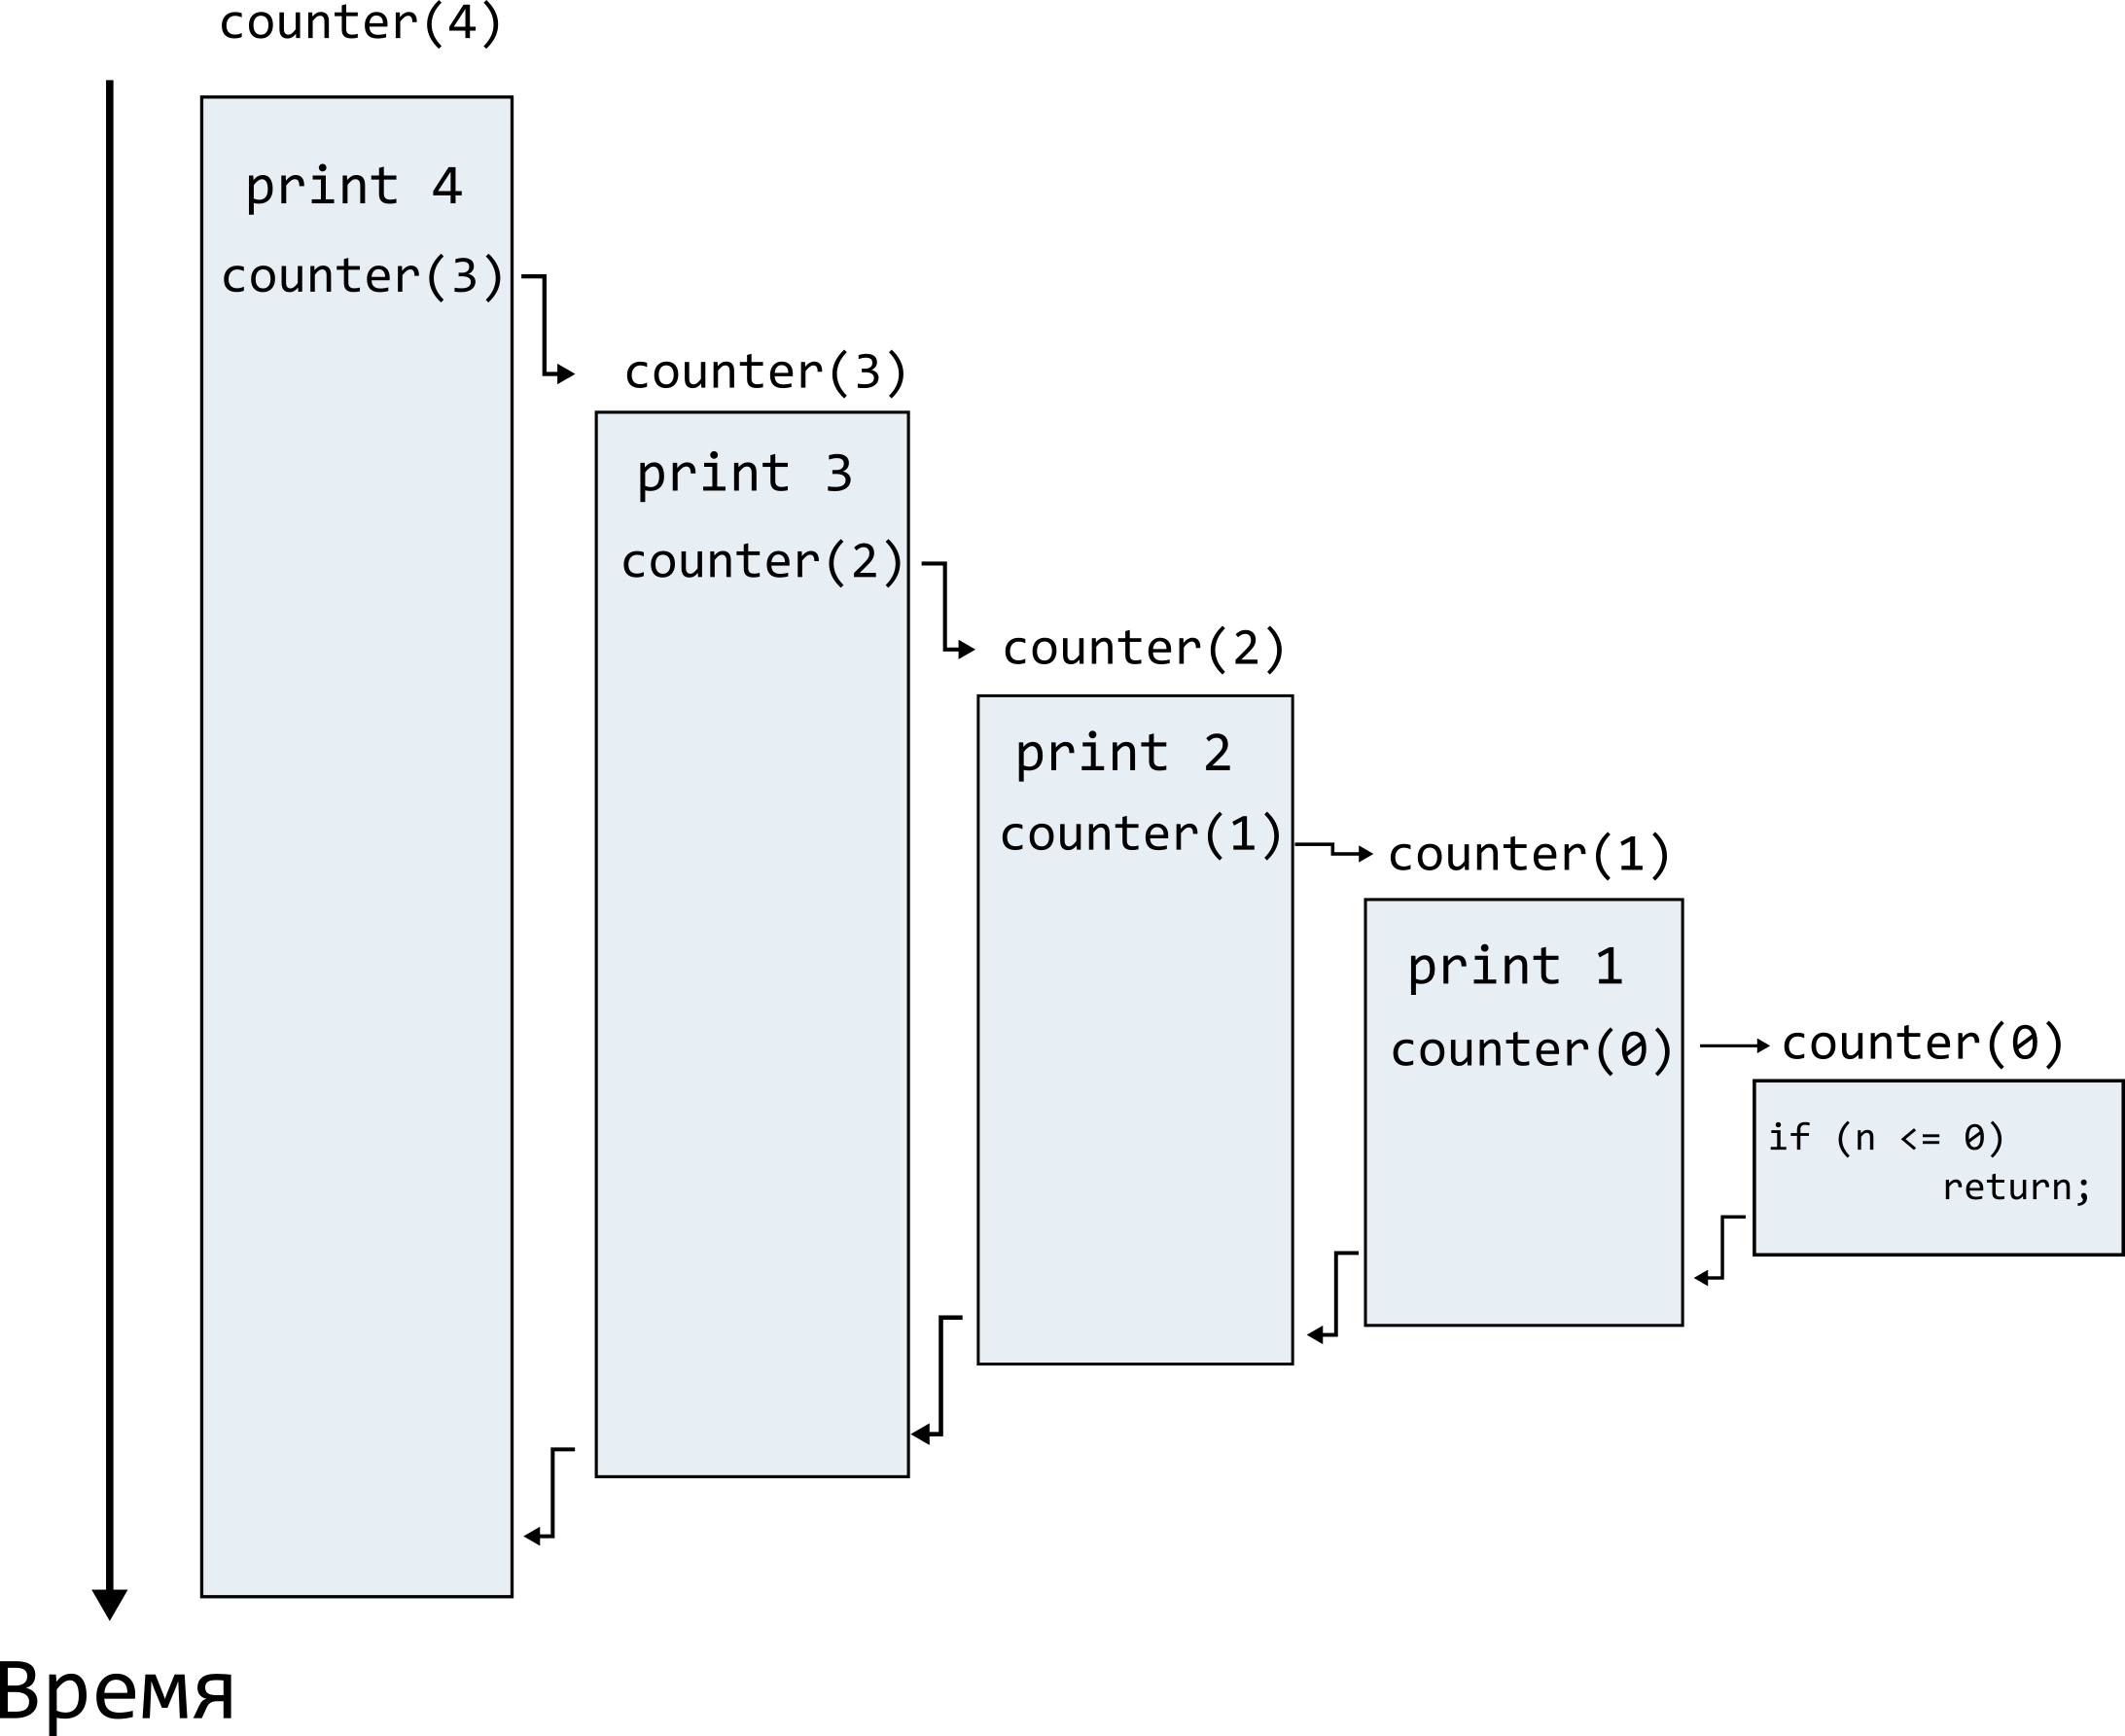
\includegraphics[scale=0.67]{../images/counterini.png}
\end{center}


\subsection*{Задачи:}
Решите задачи в папке \texttt{code/2recursion}.

\newpage
\section*{Передача массива в функцию}
Массивы можно передавать в функции. Однако, передача массива в функцию в языке \texttt{C} устроена таким образом, что узнать размер массива внутри функции нельзя. Поэтому размер массива нужно тоже передавать в функцию вместе с массивом.\\

Ещё одной особенностью передачи массива в функцию является то, что массив это единственный объект, который НЕ копируется при передаче в функцию. Вместо этого функция работает с оригинальным массивом. Благодаря этой особенности при изменении передаваемого массива внутри функции он изменится и вне функции. Это можно увидеть на примере функции \texttt{inc} в примере кода ниже.\\

Пример двух функций: одна печатает массив на экран, другая прибавляет ко всем элементам массива \texttt{1}.
\begin{lstlisting}
#include <stdio.h>

void print_array(int array[], int size) 
{
    for (int i = 0; i < size; ++i)
        printf("%i ", array[i]);
        
    printf("\n");
}

void inc(int array[], int size) 
{
    for (int i = 0; i < size; ++i)
        array[i] += 1;
}

int main() 
{
    int a[10] = {4, 8, 15, 16, 23, 42};
    print_array(a, 6);
    inc(a, 6);
    print_array(a, 6);
}
\end{lstlisting}


\subsection*{Задачи:}
Решите задачи в папках \texttt{code/3array\_to\_function} и \texttt{code/4function\_prototypes}.

\newpage
\section*{Решения задач на рекурсию}
Эту главу следует читать только после того как вы прорешаете задачи из папки \texttt{code/2recursion}.

\begin{itemize}
\item Функция \texttt{counter}, которая рекурсивно печатает числа от \texttt{n} до \texttt{1}: 
\begin{lstlisting}
void counter(int n) 
{
    if (n <= 0)
        return;
        
    counter(n - 1);
    printf("%i ", n);
}
\end{lstlisting}
Для лучшего понятия, что происходит в этой функциях \texttt{counter} рассмотрим на схемы вызовов рекурсивной функции. Для изначальной функции \texttt{counter} она выглядит следующим образом (предположим, что вызываем \texttt{counter(4)}):


\begin{center}
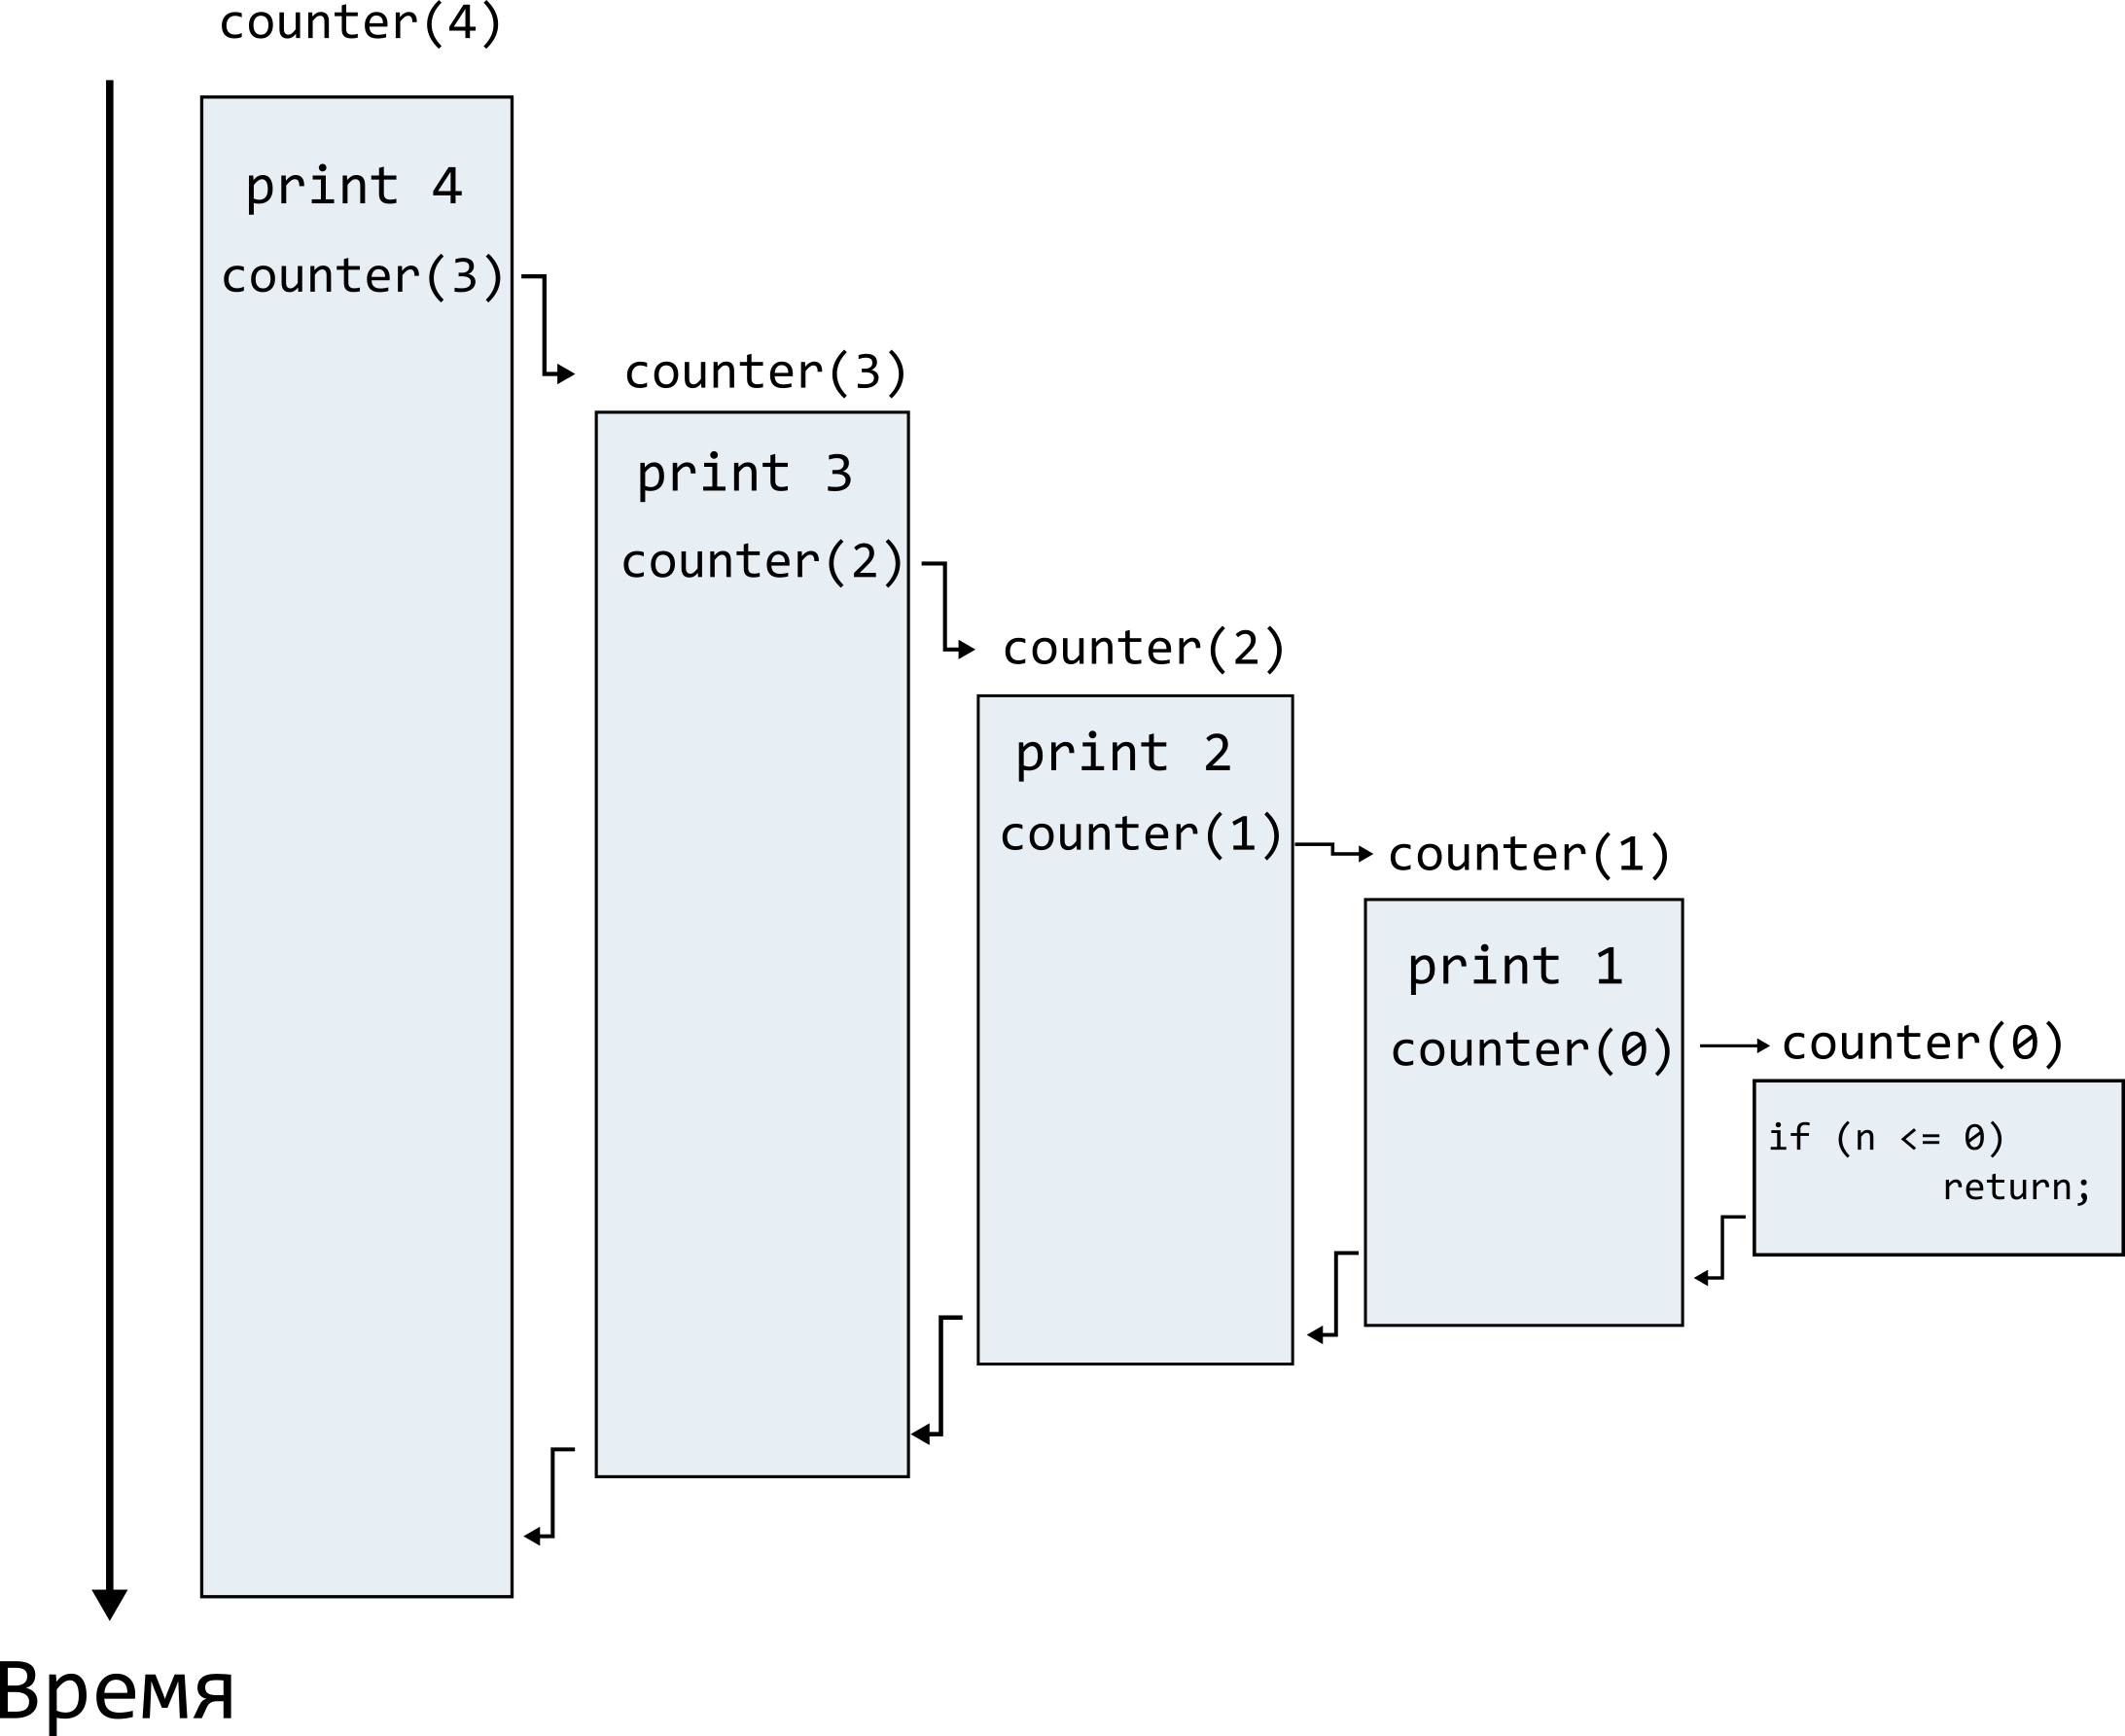
\includegraphics[scale=0.67]{../images/counterini.png}
\end{center}


\newpage

\item Немного изменим изначальную функцию \texttt{counter} чтобы она печатала числа по возрастанию от 1 до \texttt{n}:
\begin{lstlisting}
void counter(int n) 
{
    if (n <= 0)
        return;
        
    printf("%i ", n);
    counter(n - 1);
}
\end{lstlisting}
Схема для функции \texttt{counter}, которая печатает числа по возрастанию выглядит так:
\begin{center}
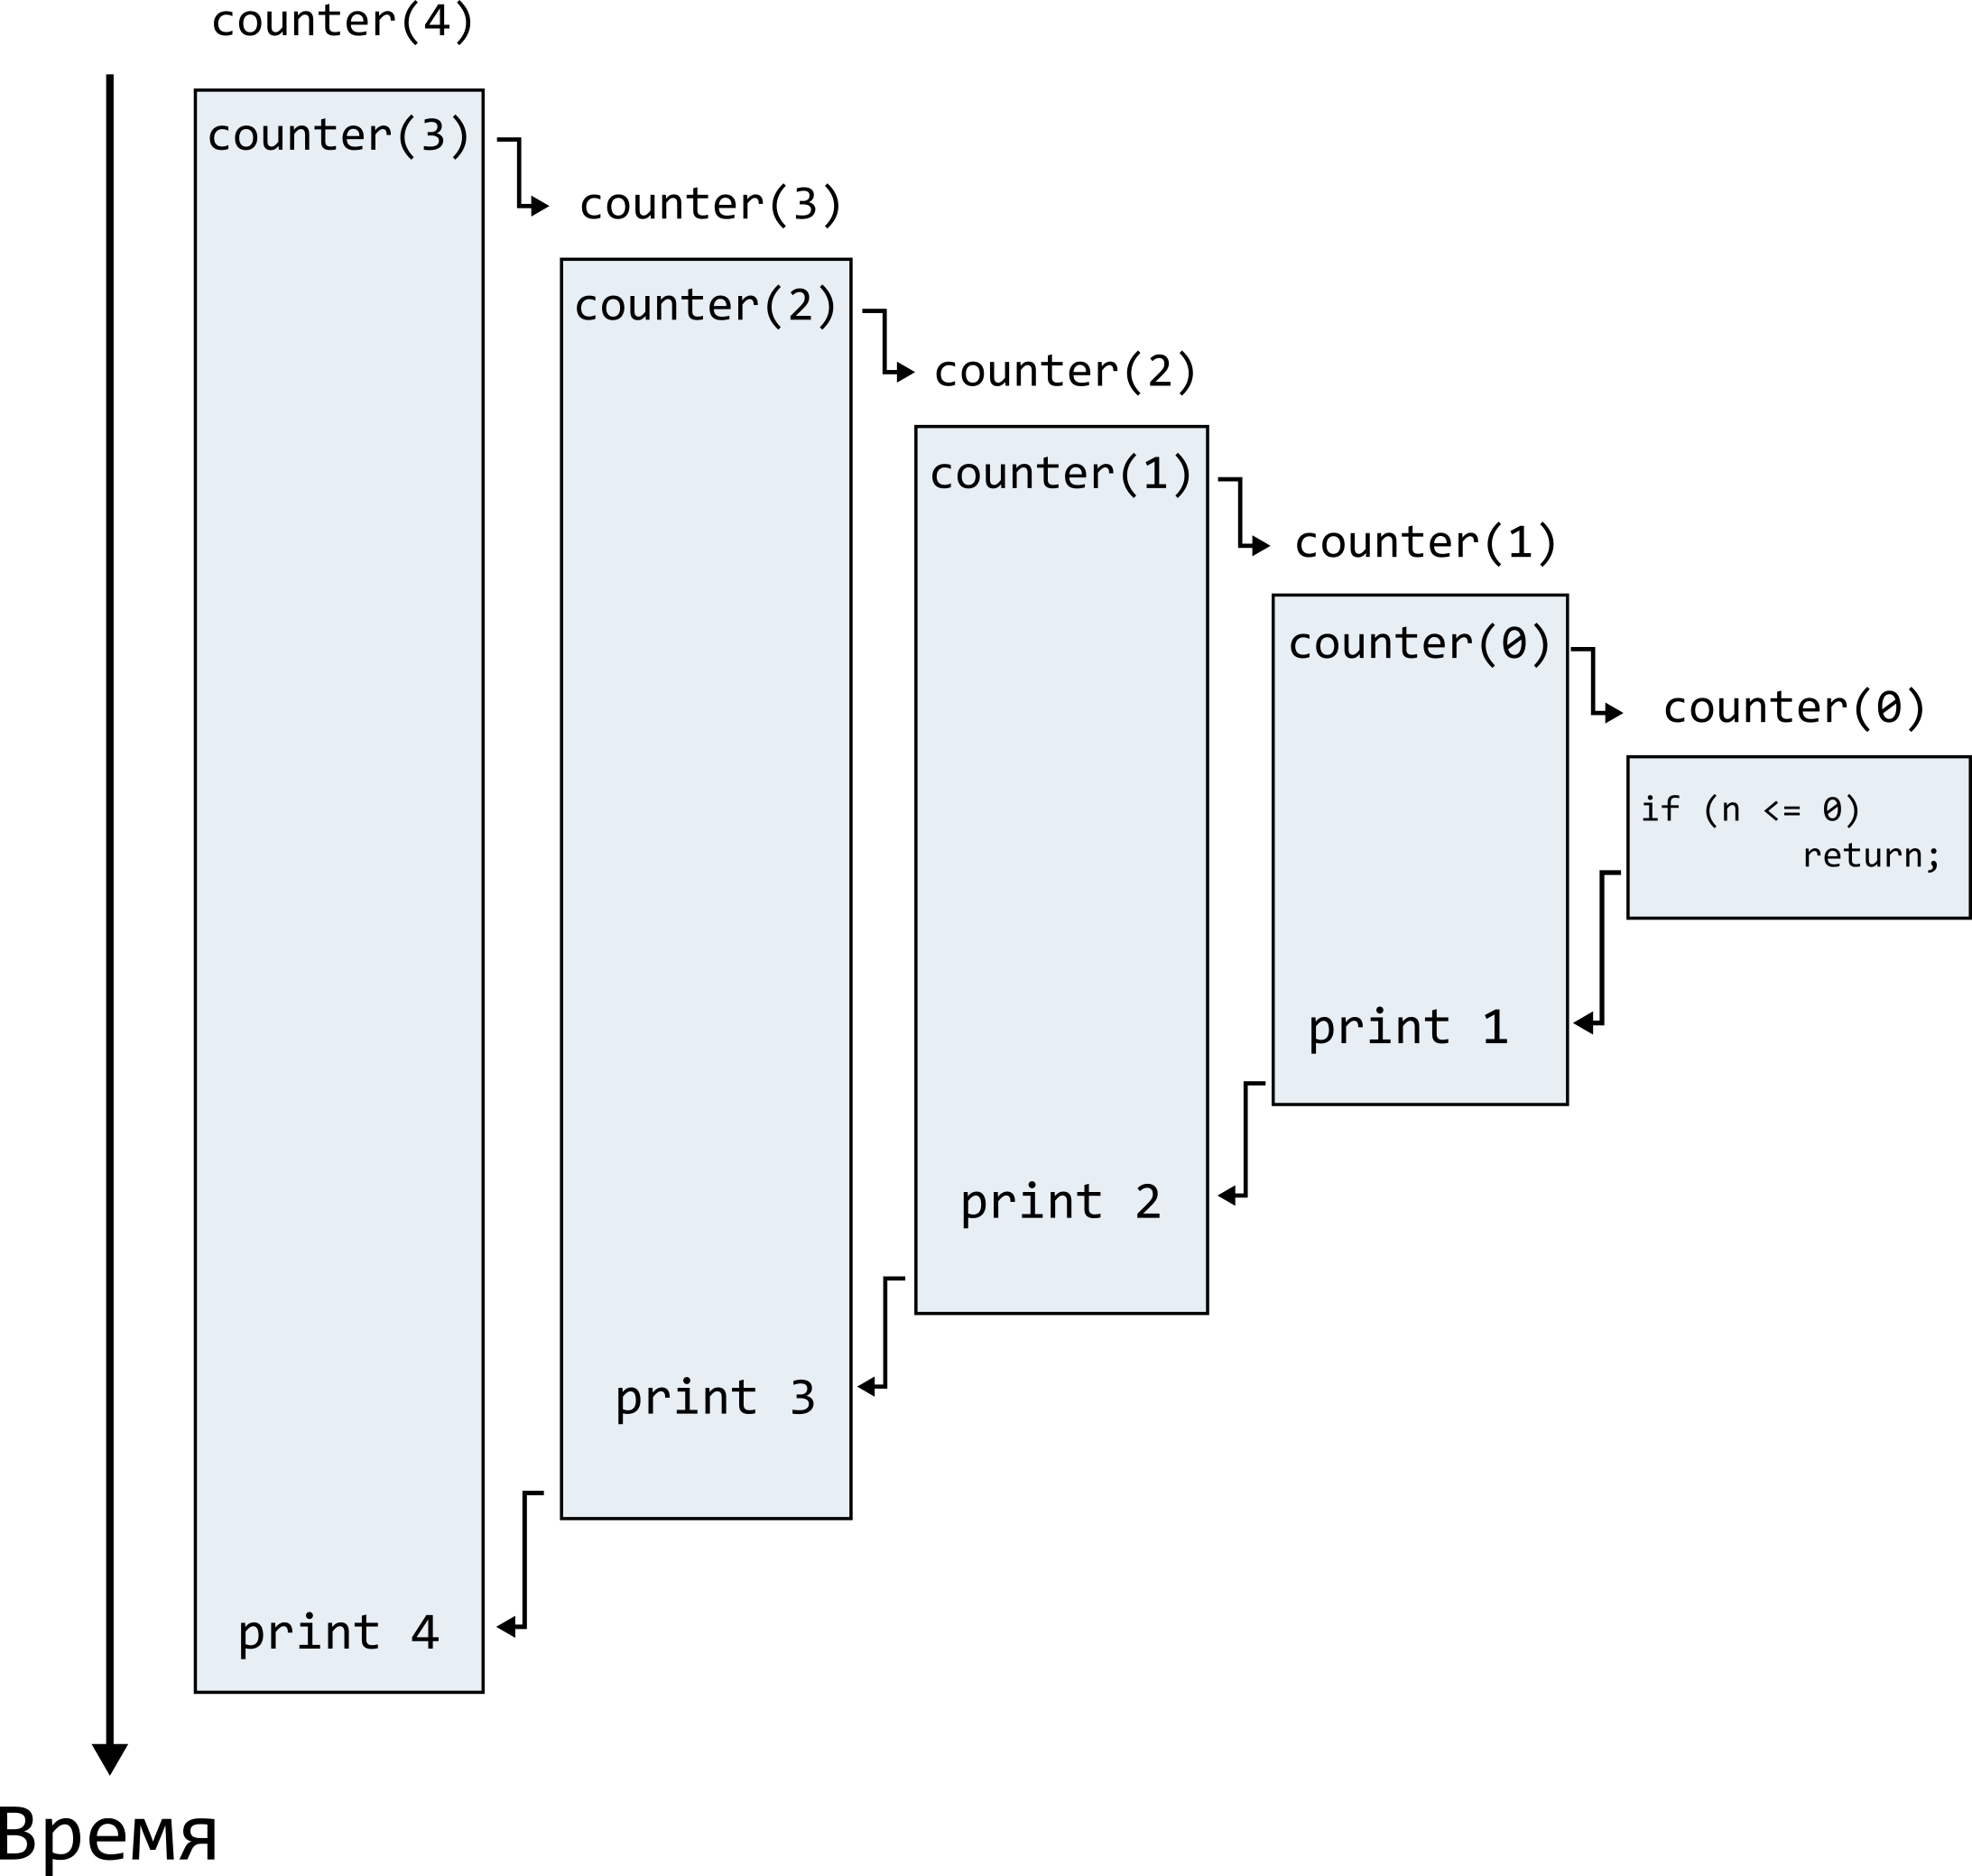
\includegraphics[scale=0.67]{../images/counter.png}
\end{center}

\newpage
\item \textbf{Скобочки:} Напишите рекурсивную функцию \texttt{brackets}, которая будет печатать некоторую скобочную последовательность. \texttt{brackets(n)} должна сначала печатать \texttt{n} открывающихся скобочек, а затем \texttt{n} закрывающихся. Например, вызов \texttt{bracket(4)} должен напечатать \texttt{(((())))}. \\
Чтобы это сделать рекурсивно нужно сделать следующее:
\begin{itemize}
\item Напечатать открывающуюся скобку
\item Напечатать \texttt{n-1} открывающихся и \texttt{n-1} закрывающихся скобок вызовом рекурсивной функции
\item Напечатать закрывающуюся скобку
\end{itemize}
\begin{lstlisting}
#include <stdio.h>

void brackets(int n) 
{
    if (n == 0)
        return;
        
    printf("(");
    brackets(n - 1);
    printf(")");
}

int main() 
{
    brackets(5);
}
\end{lstlisting}
Схема вызовов для этой функции(вызываем \texttt{brackets(3)}):
\begin{center}
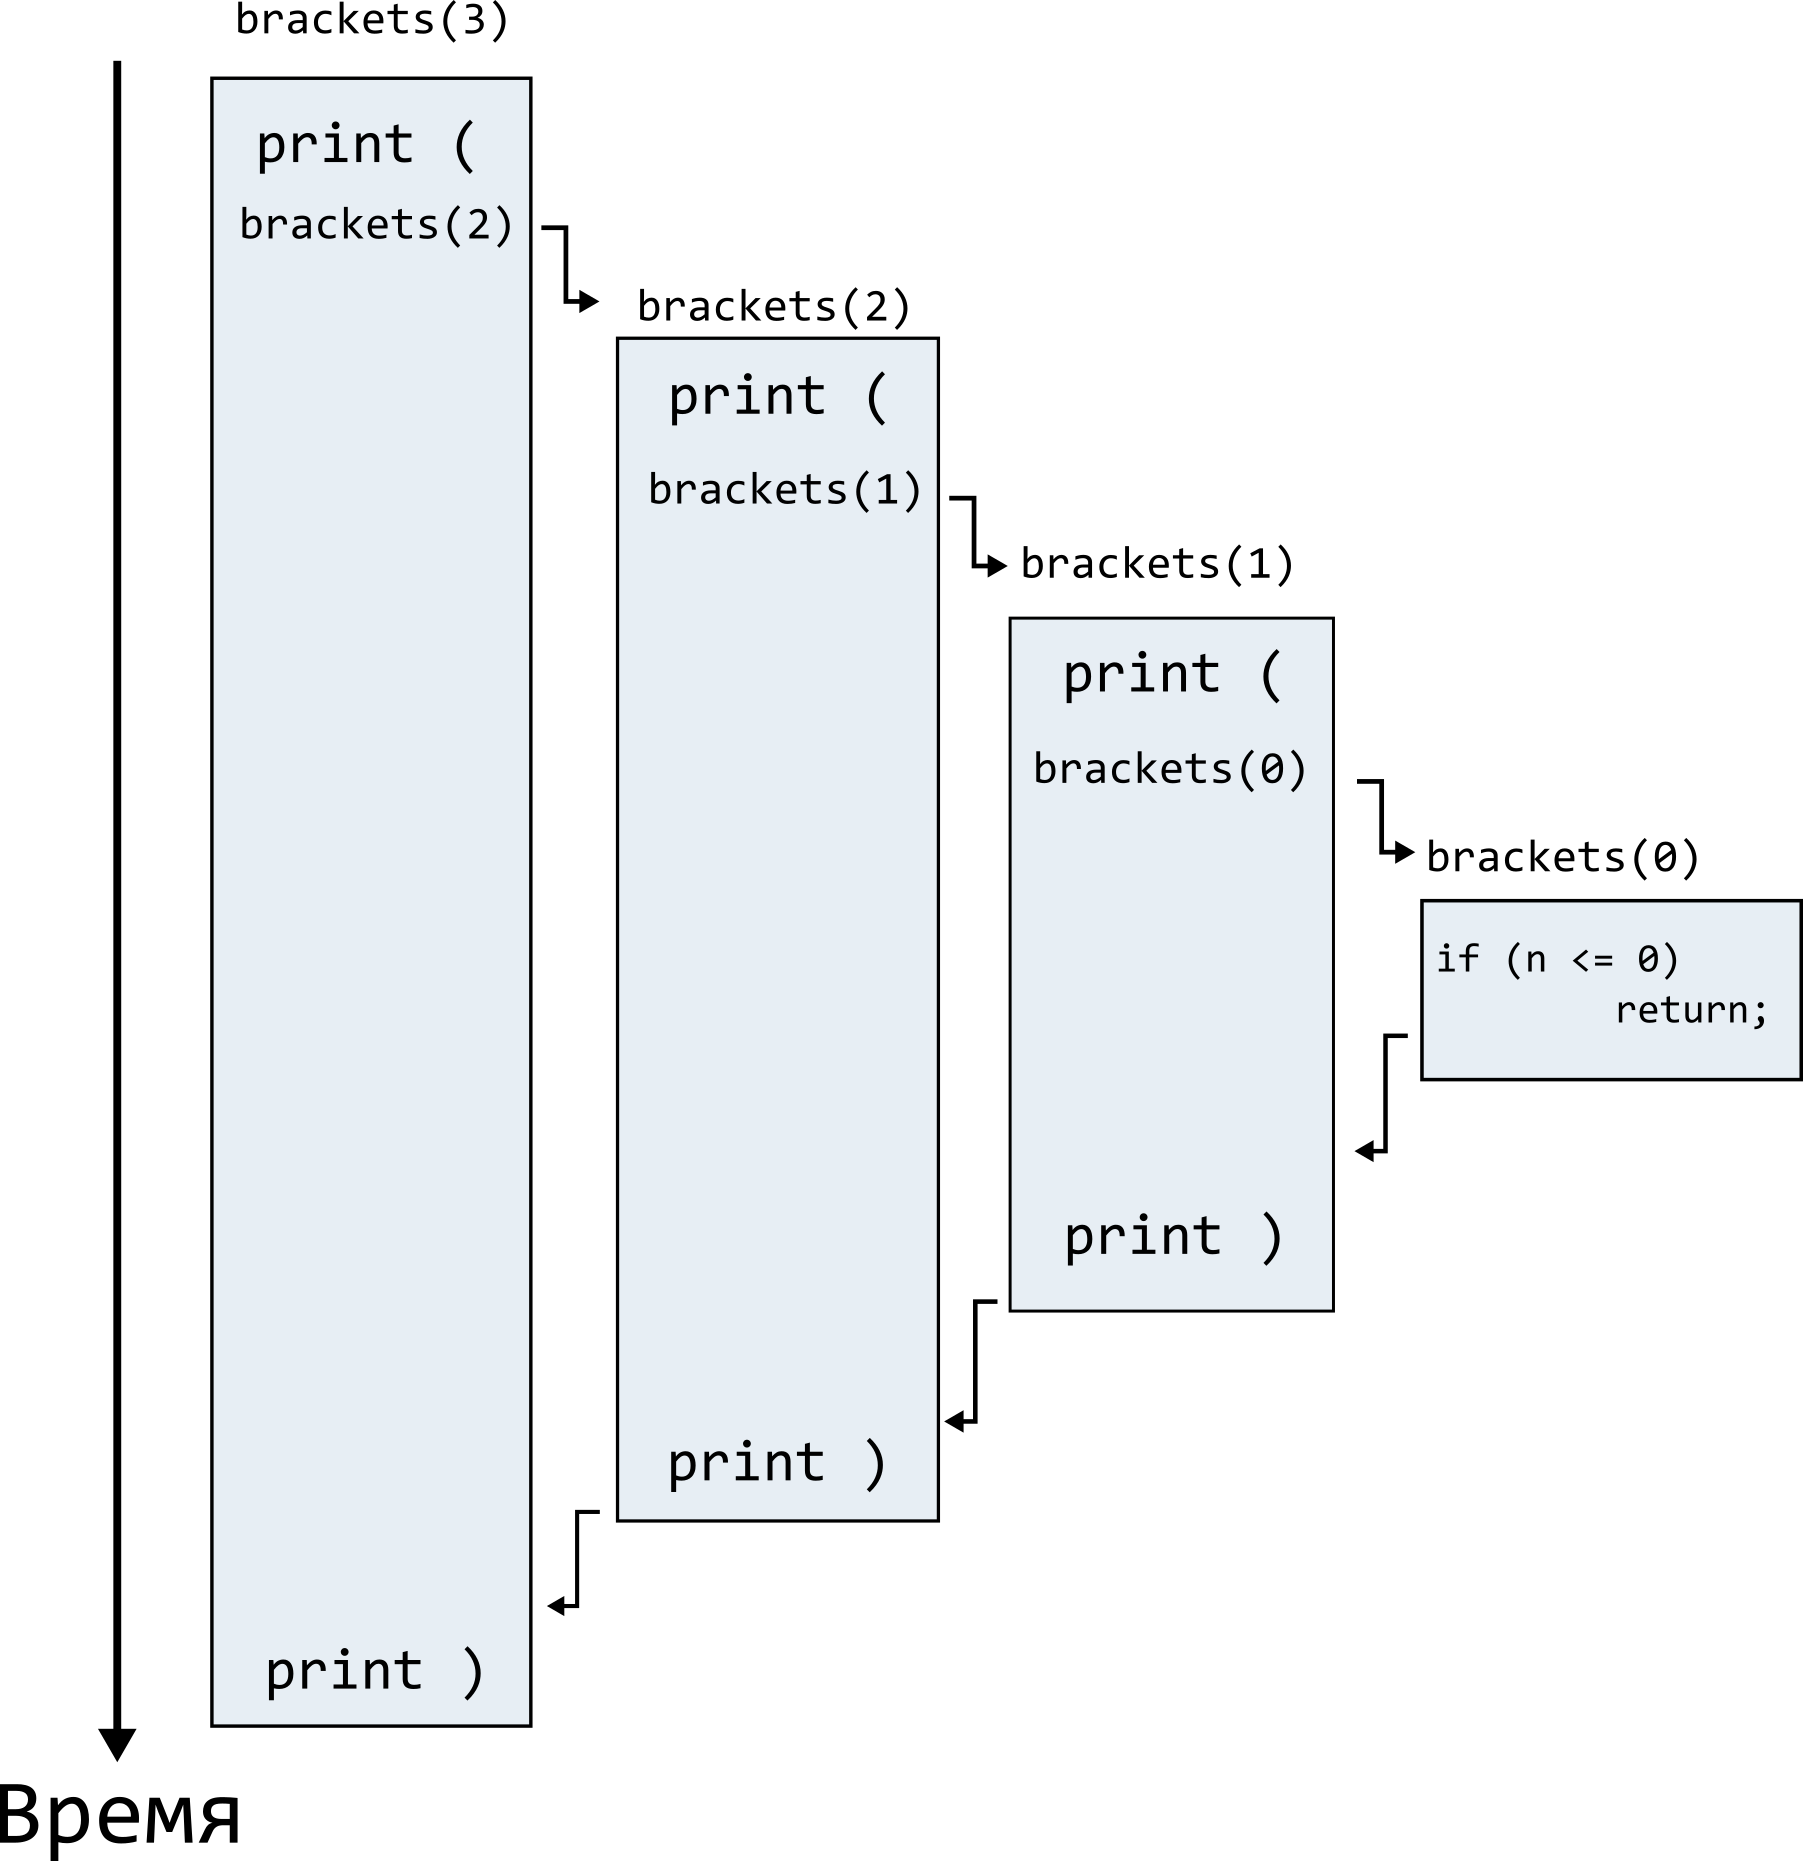
\includegraphics[scale=0.72]{../images/brackets.png}
\end{center}

\newpage
\item \textbf{Фибоначчи:}
Для вычисления числа Фибоначчи было написано 2 функции. Функция \texttt{fib} вычисляет число Фибоначчи итеративно(то есть с помощью цикла), а функция \texttt{fibrec} вычисляет то же самое рекурсивно.
\begin{lstlisting}
#include <stdio.h>

int fib(int n) 
{
    int a = 0, b = 1;
    for (int i = 1; i < n; ++i) 
    {
        int temp = a + b;
        a = b;
        b = temp;
    }
    return b;
}

int fibrec(int n) 
{
    if (n < 2)
        return n;

    return fibrec(n - 1) + fibrec(n - 2);
}
int main() 
{
    printf("%i\n", fib(45));
    printf("%i\n", fibrec(45));
}
\end{lstlisting}
Кажется, что обе функции работают, но почему-то рекурсивная функция работает намного медленней.
Почему это происходит? \\

\textit{Замечание}: Это не связано с переполнением числа. 45-е число Фибоначчи может храниться в переменной типа \texttt{int}.


\newpage
Рекурсивная функция вычисления чисел Фибоначчи работает так медленно потому что она по многу раз вычисляет одни и те же значения. На изображении ниже предсталена схема вызовов этой функции для вычисления 10-го числа Фибоначчи.
\begin{center}
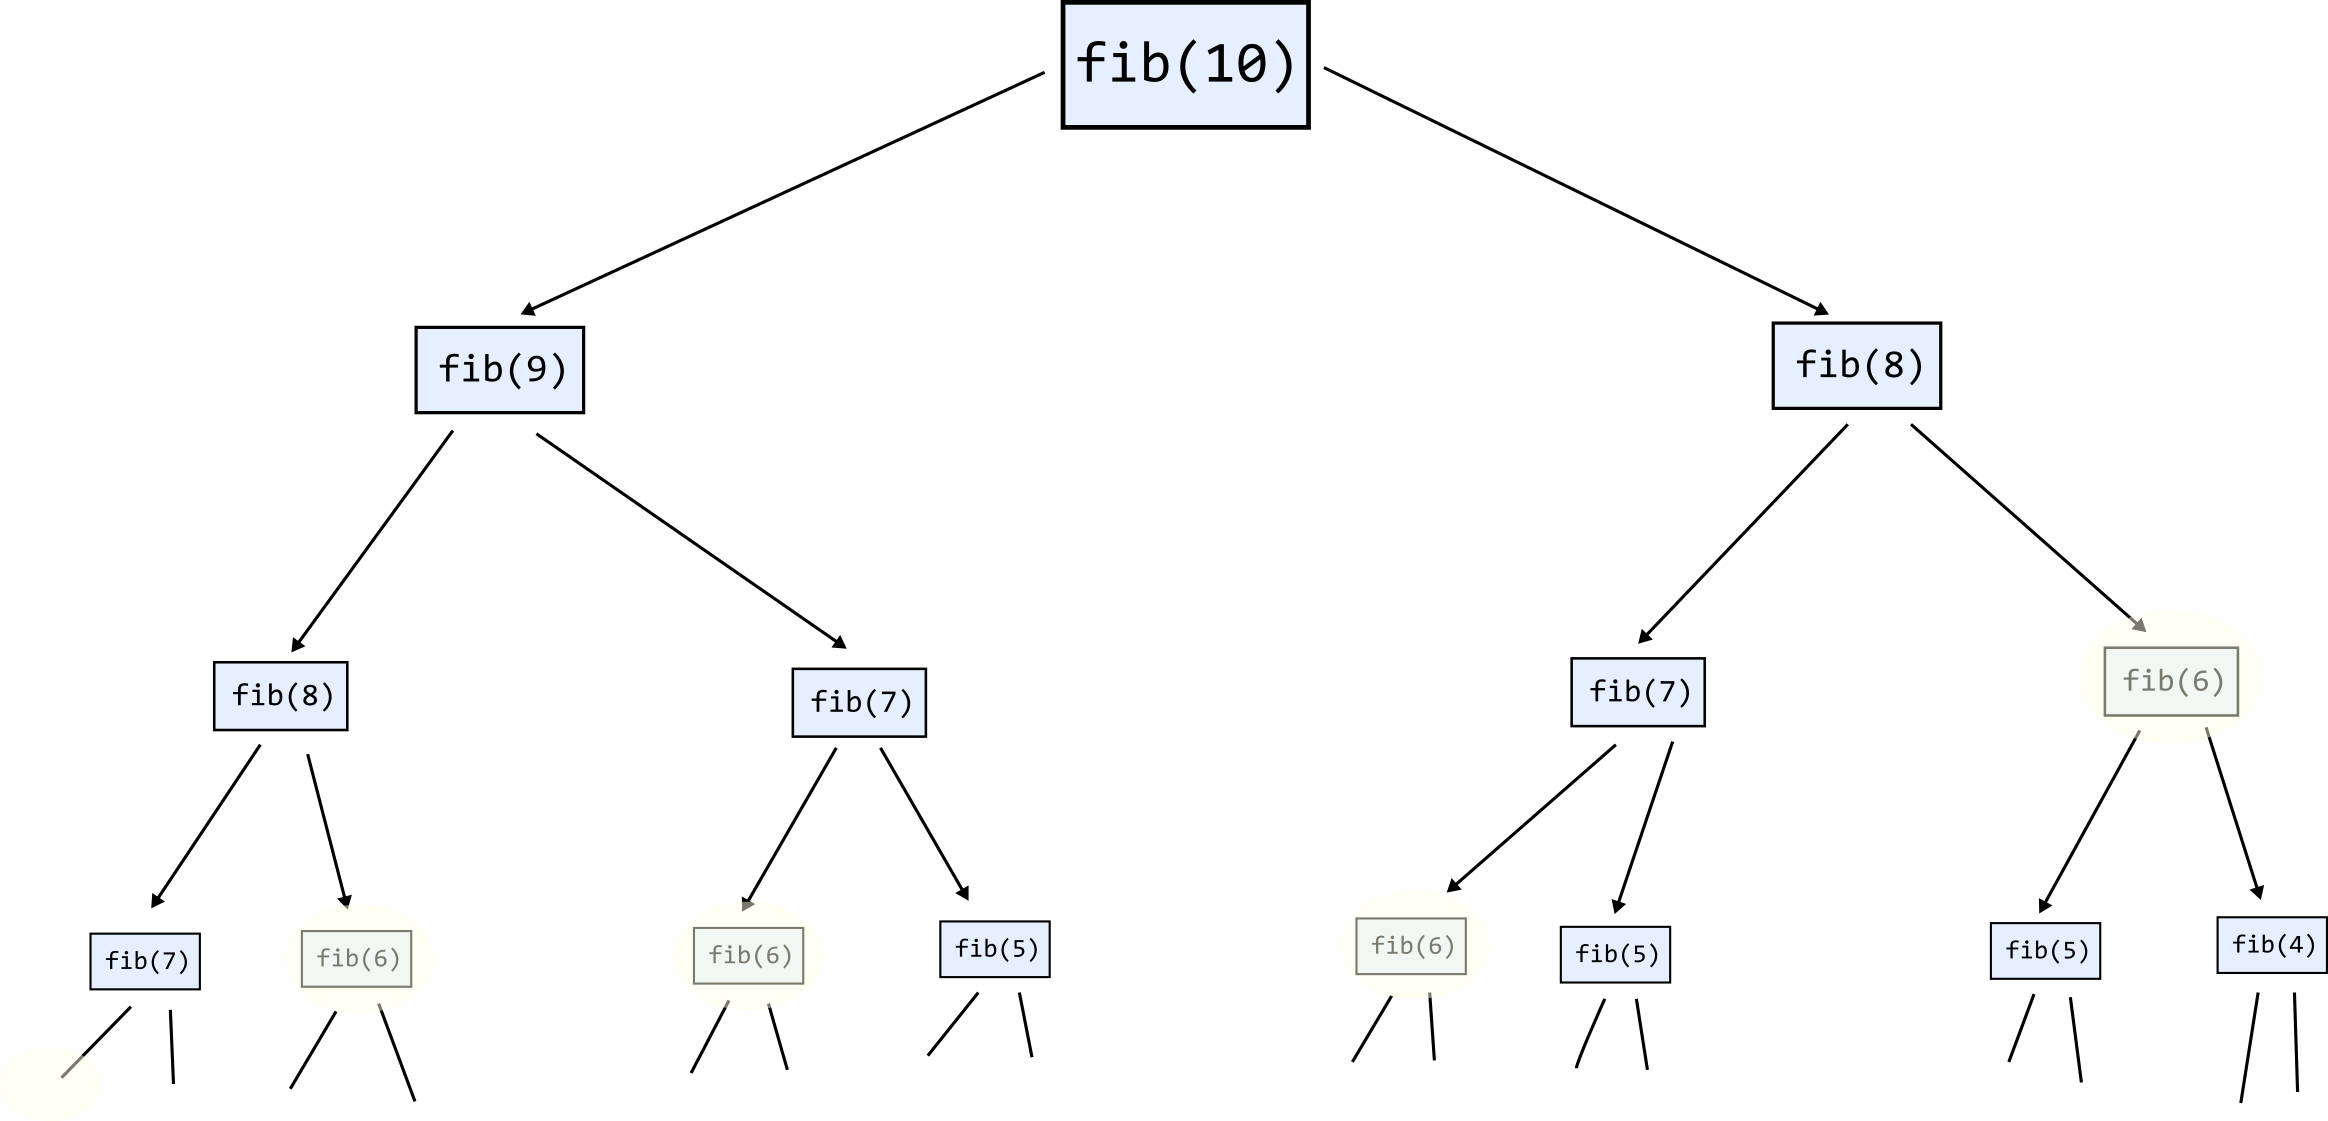
\includegraphics[scale=0.8]{../images/fib.png}
\end{center}
Видно что промежуточные числа Фибоначчи вычисляются заново по много раз. Например, \texttt{fib(6)} вызывается 5 раз в процесе вычисления \texttt{fib(10)}, \texttt{fib(5)} вызывается 8 раз, а меньшие числа Фибоначчи вычисляются ещё чаще. Получается, что количество операций для вычисления одного числа Фибоначчи рекурсивным способом экспоненциально большое.\\

Рекурсивную функцию можно исправить если в процессе выполнения запоминать все промежуточные вычисления и не делать их заново. Для этого заведём глобальный массив \texttt{data} в котором будем хранить все промежуточные числа Фибоначчи. В начале все элементы этого массива равны нулю. Теперь мы продолжаем рекурсию только если мы не вычисляли данное число ранее и \texttt{data[n] == 0}.

\begin{lstlisting}
#include <stdio.h>

int data[1000];

int fibrec(int n) 
{
    if (n < 2)
        return n;

    if (data[n] == 0)
        data[n] = fibrec(n - 1) + fibrec(n - 2);

    return data[n];
}

int main() 
{
    printf("%i\n", fibrec(45));
}
\end{lstlisting}

\end{itemize}


\end{document}
